\section{RF Layer and Channel Models}
\label{sec:rf}

Two channel models coexist.  The audio-domain simulator
(\texttt{channel.py}) is the article's model --- timing offset, CFO
with quadratic drift, optional Rayleigh fading, multipath
$[1,0,0.4,0,0,0.2]$, AWGN, BSC block flips ($p=10^{-3}$) and BEC block
erasures ($p=2\cdot 10^{-2}$) --- and drives most sweeps.  The RF
layer (\texttt{rf.py}) models the actual transceiver chain, so carrier
offsets \emph{emerge from oscillator physics} instead of being
injected as parameters.

\subsection{The SSB Chain}

Simulation runs at a 48\,kHz IF rate with a 12\,kHz carrier standing in
for the RF carrier; LO errors are specified in ppm of the nominal RF
frequency (e.g.\ 7.1\,MHz), so audio-band offsets come out physically
correct (Figure~\ref{fig:rf_chain}).

\begin{figure}[H]
    \centering
    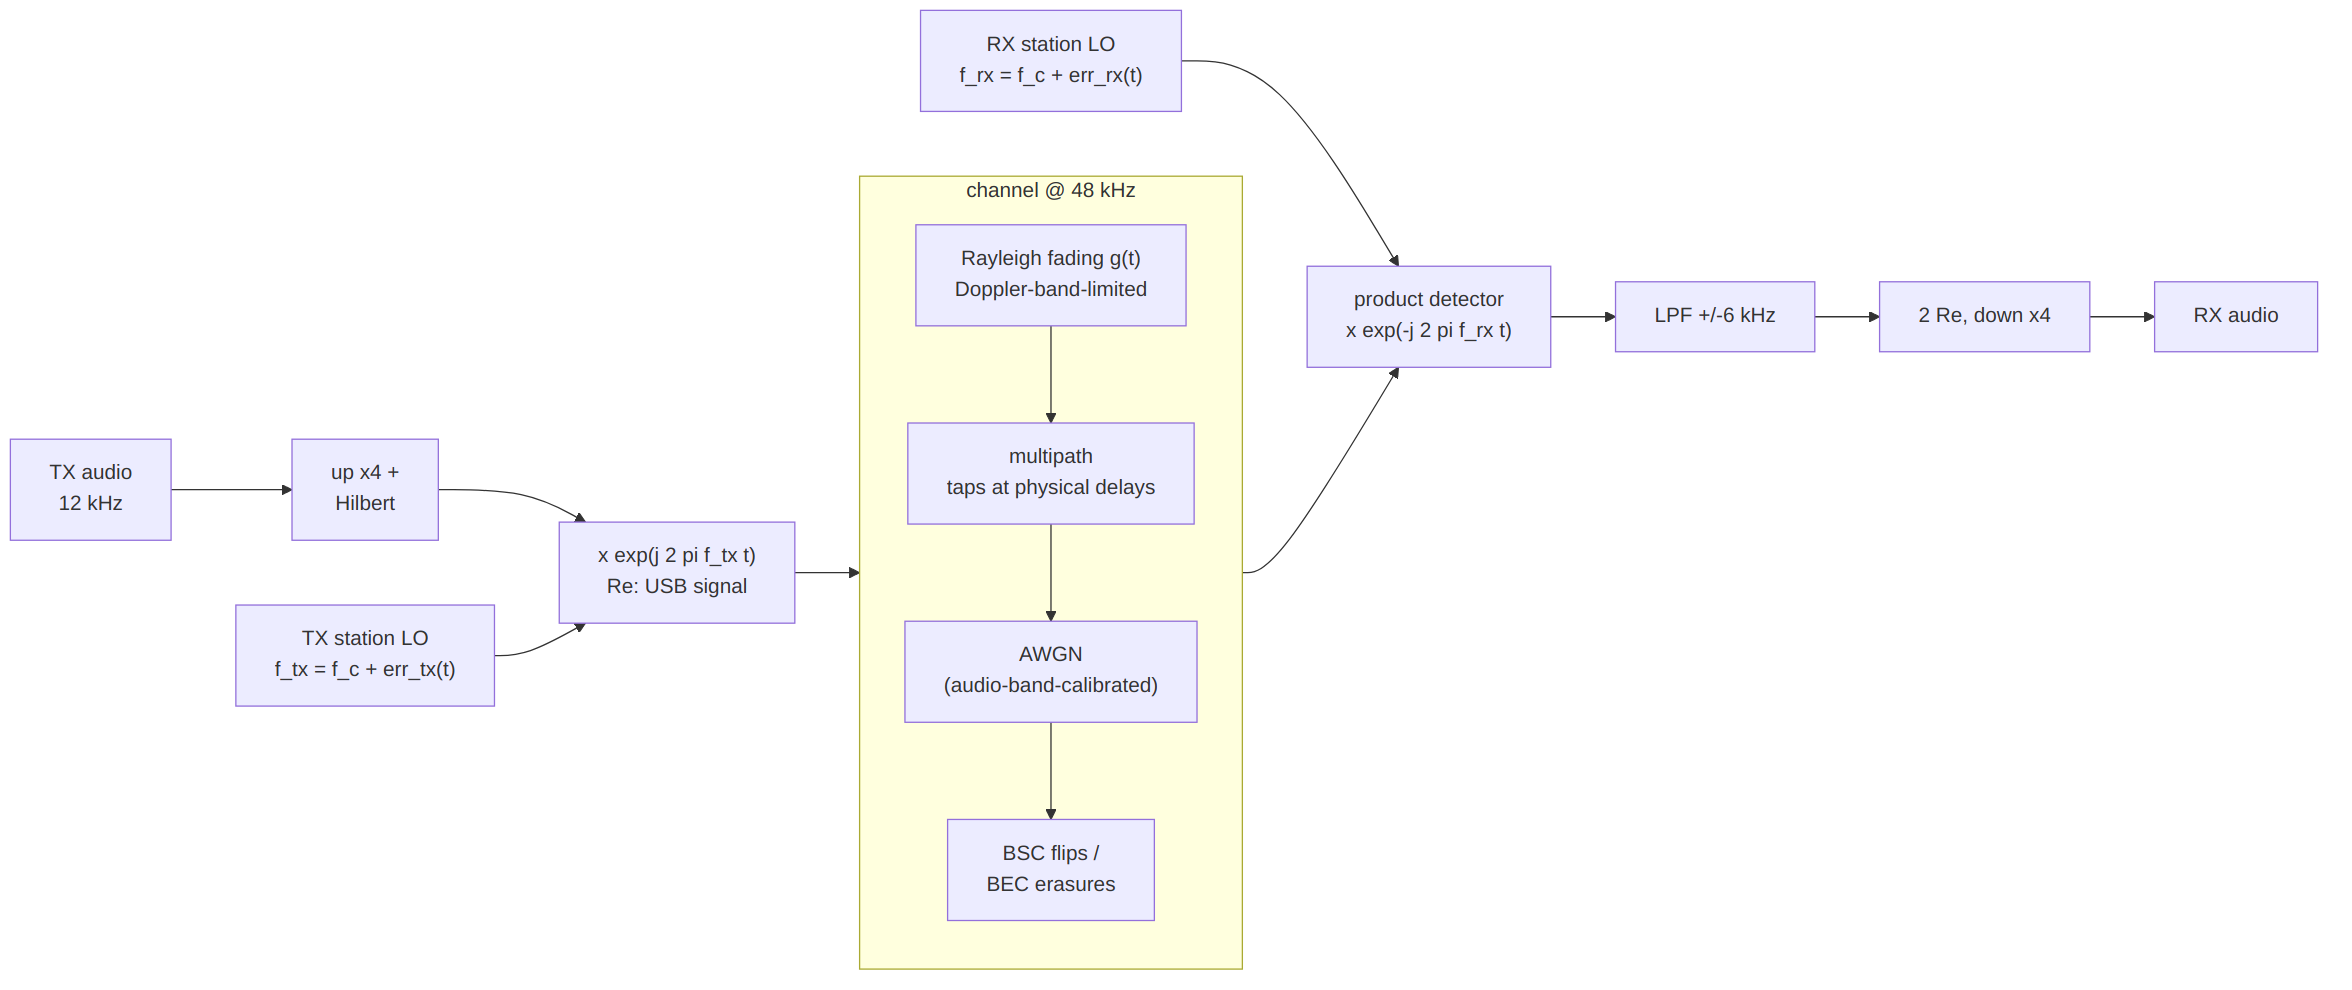
\includegraphics[width=\textwidth]{images/rf_chain.png}
    \caption{The RF chain: USB modulator, 48\,kHz channel (fading,
             multipath, AWGN, BSC/BEC), product detector.}
    \label{fig:rf_chain}
\end{figure}

\subsection{The LO Model}

Each \texttt{StationRF} has \emph{one} reference oscillator shared by
its TX and RX, as in a real transceiver:
\[
    \mathrm{err}(t) \;=\; f_{\mathrm{rf}} \cdot \mathrm{ppm} \cdot
    10^{-6} \;+\; \mathrm{drift}_{\mathrm{Hz/s}} \cdot t \;+\;
    \mathrm{trim}_{\mathrm{Hz}},
\]
and the audio CFO between two stations is
$\mathrm{err}_{tx}(t) - \mathrm{err}_{rx}(t)$
(Figure~\ref{fig:lo_model}).  Validated against the modem's own CFO
measurements to 0.1\,Hz at $+99.4$, $-106.5$, and $+284.0$\,Hz
scenarios.  \texttt{trim\_hz} is the AFC hook of
Section~\ref{sec:afc}.

\begin{figure}[H]
    \centering
    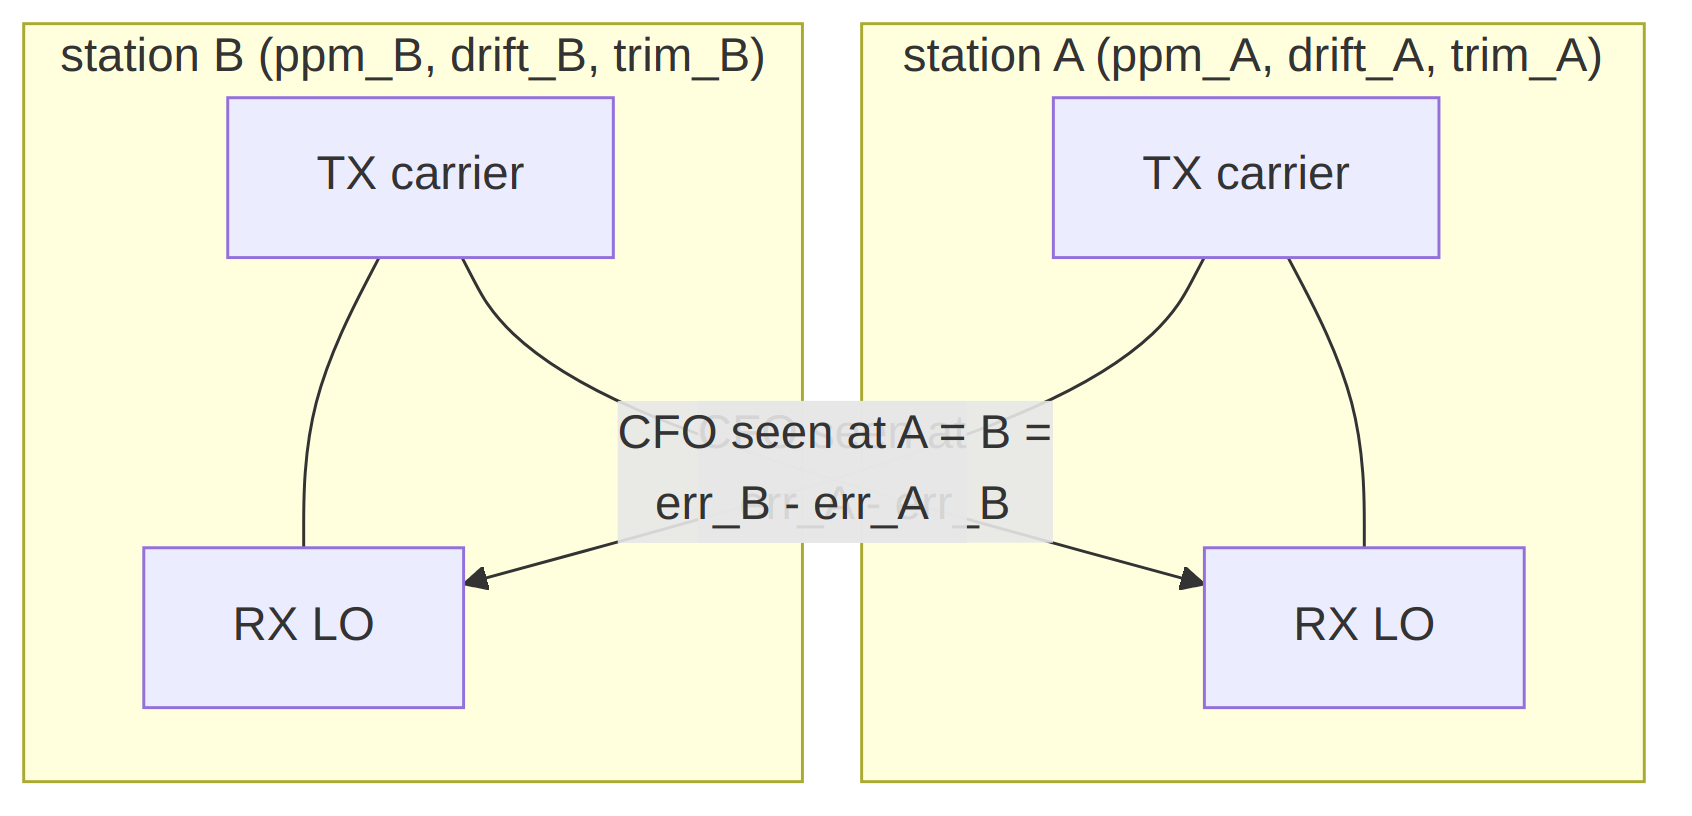
\includegraphics[width=0.75\textwidth]{images/lo_model.png}
    \caption{Per-station shared-reference LO model: where CFO comes
             from.}
    \label{fig:lo_model}
\end{figure}

\subsection{Calibration Subtleties}

Three traps are documented in code comments because each silently
costs dB if gotten wrong:

\begin{itemize}
    \item \textbf{AWGN sizing.}  The product detector's
          $\mathrm{Re}(\cdot)$ halves \emph{uncorrelated noise} power
          but not the coherent signal, so the RF noise variance factor
          is $2 \cdot P_{\mathrm{sig}} \cdot 10^{-\mathrm{SNR}/10}$
          --- not the naive bandwidth ratio, which is 3\,dB off.  With
          the correct factor the audio-band SNR convention matches the
          audio-domain simulator, so all measured sensitivities carry
          over (9/10 decodes at $-5$\,dB through the full RF chain).
    \item \textbf{Rayleigh fading.}  Complex Gaussian band-limited to
          the Doppler bandwidth (0.1--0.5\,Hz, typical HF QSB), unit
          mean power, applied to the analytic signal; AWGN is sized
          from the \emph{average} faded power, so instantaneous SNR
          swings around the nominal value.
    \item \textbf{Multipath at RF.}  The audio-domain tap delays are
          physical, so taps map to interpolation-factor-spaced
          positions at the RF rate.
\end{itemize}

\subsection{The Recorded Demonstration}

\texttt{experiments/demo\_wav.py} records a complete two-station
session through this chain: station A at $+6$\,ppm and B at $-8$\,ppm
on 7.1\,MHz (A$\rightarrow$B CFO $\approx +99.4$\,Hz, handled
invisibly by the protocol).  The output WAV is the audio of a
\emph{passive monitor} receiver with its own $+2$\,ppm LO --- A's
frames appear at $\approx +28$\,Hz and B's at $\approx -71$\,Hz in the
blind-decoded transcript (Appendix~\ref{app:demo}), per-station CFO
fingerprints with the thermal drift visible across the session.
